

\frame{\frametitle{A question !}
   \begin{itemize}[<+->]
	\item  Herein lies the crux of science processing problems for me …
\item In a meeting in 2007 I was asked :
   \end{itemize}
\begin{center}
   “What do you think you are doing, a science project or something ?” \\
   “Well yes … I rather think I am!” \\
\end{center}
did not seem to be the expected answer.
}


\frame{\frametitle{ Is science processing different ?}
   \begin{itemize}
	\item To clarify In the ESA context think “different to satellite development” 
\item i.e. the waterfall
   \begin{itemize}
\item Requirements
\item Design
\item Implement
\item Deliver
   \end{itemize}
\item Precisely in that order and precisely once
\item Genuinely how many of you ever do this ?
\item Not clear any large software is done in this manner anymore
   \end{itemize}
}


\frame{\frametitle{Methodology Timeline}
\begin{itemize}
\item OO Development Methodology Timeline
\end{itemize}
\begin{center}
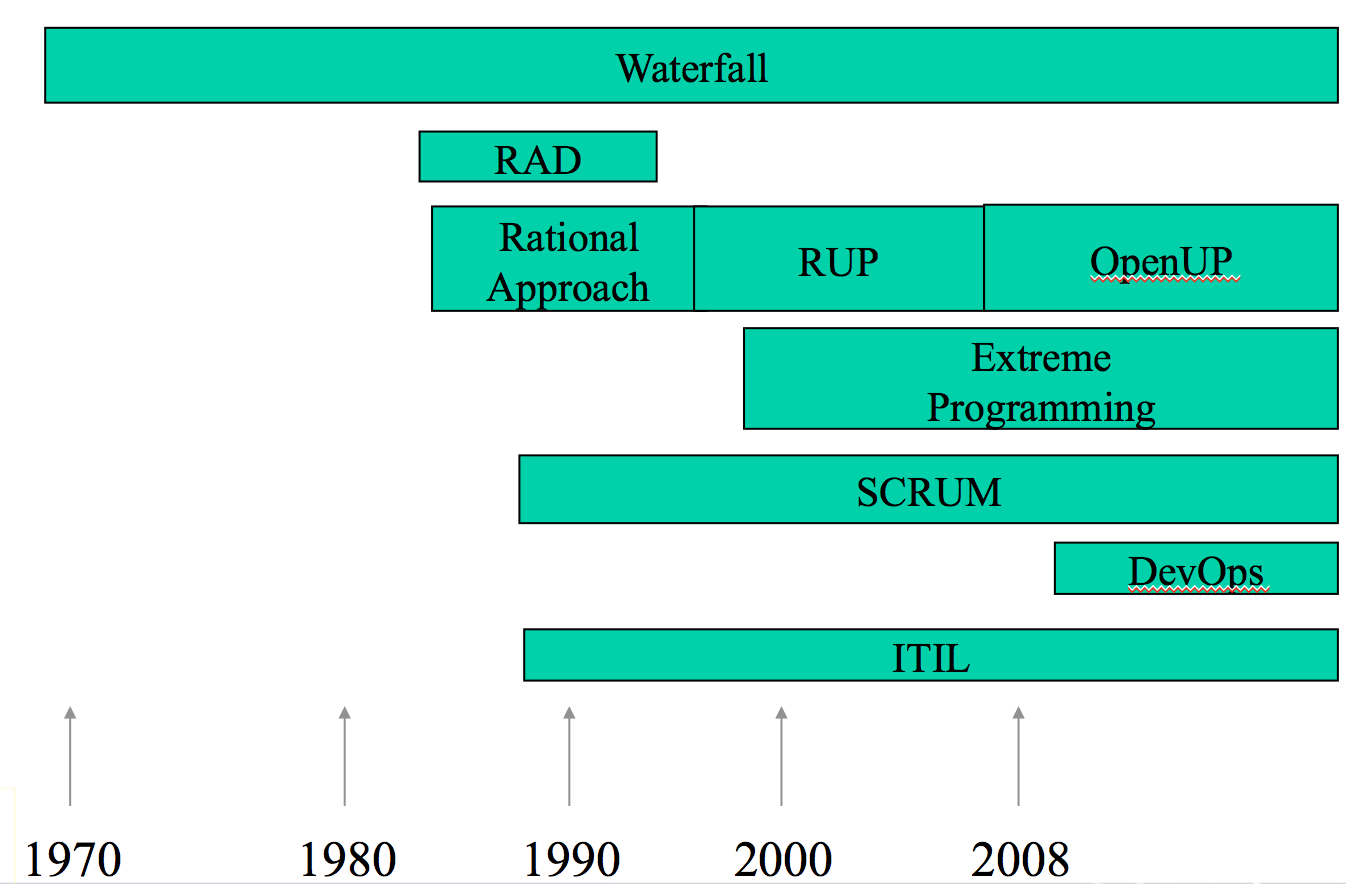
\includegraphics[width=0.8\textwidth]{images/ootimeline}
\end{center}
}

\frame{\frametitle{RAD and RUP evolve}
\begin{itemize}
\item Problems with Traditional Waterfall
\begin{itemize}
\item Customer doesn't see results for a long time
\item Sometimes delivery is not what was wanted
\item Often the requirements have changed
\item Especially when the customer sees the implementation
\end{itemize}
 \item Enter Iterative methodologies

\end{itemize}
\begin{center}
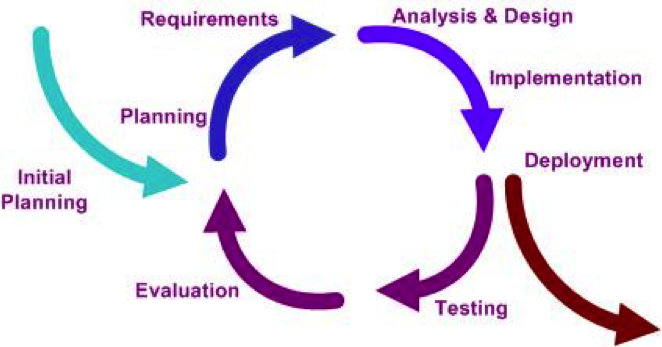
\includegraphics[width=0.7\textwidth]{images/iter}
\end{center}
{\tiny \bf from Paul Parsons}
}

\frame{\frametitle{A little amusing history .. }
\begin{itemize}
\item Royce \citep{royce70}. 
\item Considered inventor of term waterfall (his fig)
\end{itemize}
\begin{center}
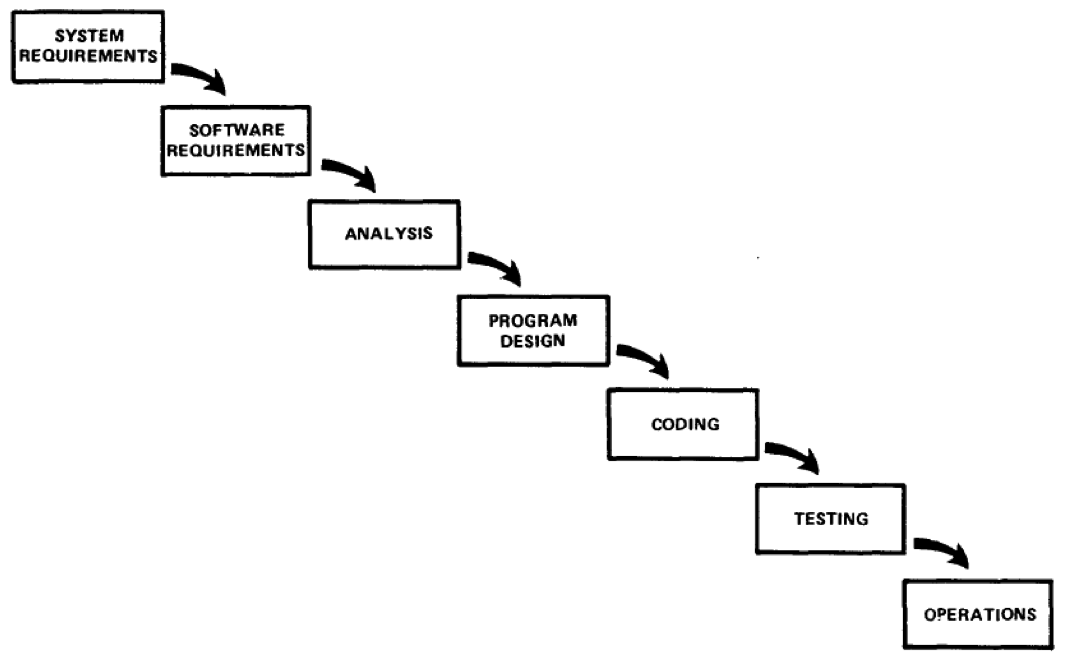
\includegraphics[width=0.8\textwidth]{images/wfall}
\end{center}
}

\frame{ \frametitle {And what is amusing \ldots }
\begin{itemize}
\item for the managers that actually read the next page of the paper 
\end{itemize}
\vspace{-5pt}
  \begin{tikzpicture} 
 \node (wf) {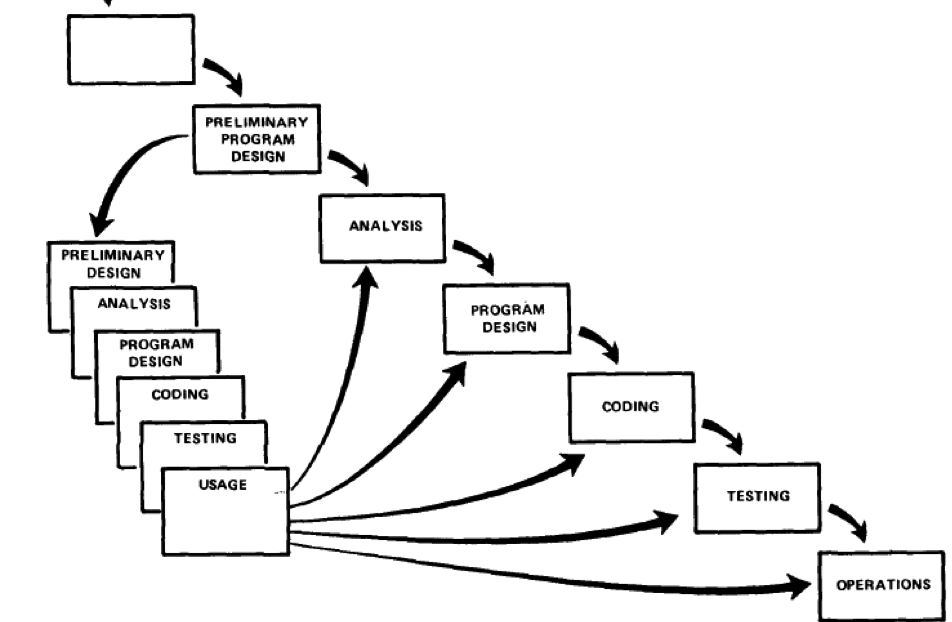
\includegraphics[width=0.8\textwidth]{images/wflaw} };
 \node (p) [right=-0.3cm of wf] {};
 \node (db) [above=1.65cm of p] {};
 \node (o) [below=0.1cm of db.south] {\color{red} Royce claims waterfall is flawed };
 \node (o2) [below=0.1cm of o.south] {\color{red} and says we should do it twice! };
 \node (o3) [below=0.1cm of o2.south] {\color{red} i.e. iterate (his other fig)
};
  \end{tikzpicture}


}

\frame{\frametitle{Agile techniques}
\begin{itemize}
\item Do things faster and cheaper with nimble teams
\begin{itemize}
\item eXtreme Programming (more to come)
\item SCRUM – huddle and watch the backlog
\item CystalClear – Cockburns’s undisciplined XP
 \item several others …
\end{itemize}
\item Rapid Application Development (RAD) does not cut it in Agile –
\begin{itemize}
\item James Martin seen as the “father of Agile”
\item but he did not go to Utah 
%snowbird meetign in Utah 2001 .. 

\end{itemize}

\end{itemize}
}

\frame{\frametitle{Extreme Development approach}
\begin{itemize}
\item One of the so called Agile techniques
\item This is not how it is ….
\end{itemize}
\begin{center}
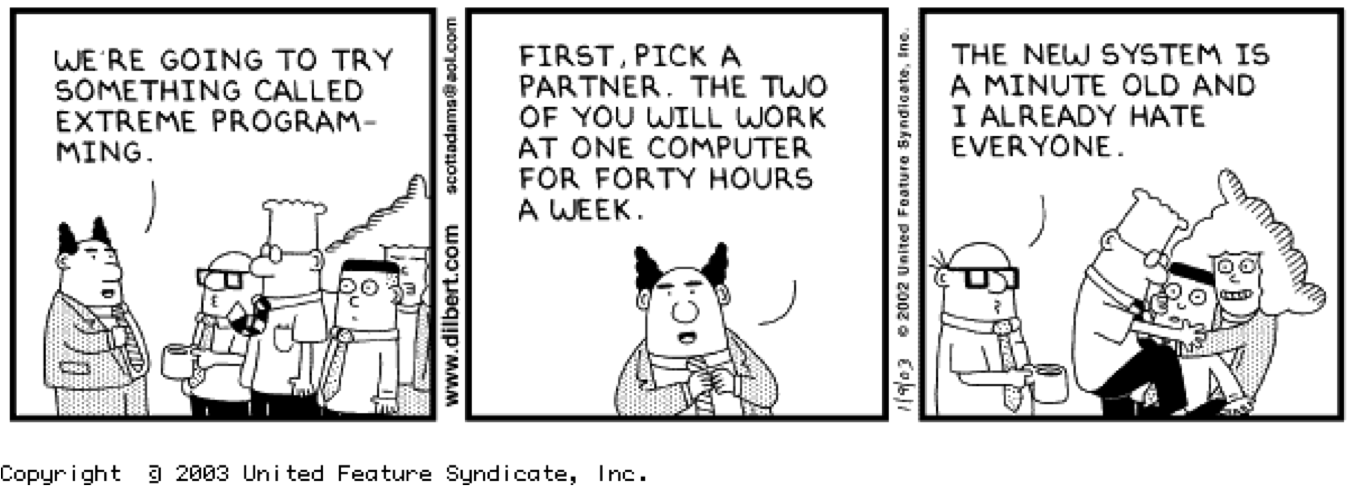
\includegraphics[width=0.8\textwidth]{images/dilbertxp}
\end{center}
}

\frame{\frametitle{eXtreme Programming}

\begin{itemize}
\item Some say nothing new started in 1950:
\begin{itemize}
\item Larman, C., Basili, V.R., 2003, IEEE Computer, http://www2.umassd.edu/SWPI/xp/articles/r6047.pdf
\end{itemize}
\item eXtreme Programming or XP was created by Kent Beck during his work on the Chrysler Comprehensive Compensation System (C3) payroll project around 1997
\item in October 1999, Extreme Programming Explained was published 
\begin{itemize}
\item Several other books followed
\item And many tools (which you already use)

\end{itemize}
\end{itemize}
}


\frame{\frametitle{Principles of XP}
\begin{itemize}
   \item Principally reduce the cost of change
\begin{itemize}
 \item Actually keep cost fixed while adapting the system
\item Embrace change !!
\end{itemize}
\item Communication 
\begin{itemize}
 \item light documentation \& metrics
\end{itemize}
\begin{itemize}
\item Simplicity  - KISS principle
\item Feedback
\item From the code via unit tests
\item From the customer {\color{green} (product owner - scientist)} via acceptance tests
\item From the team by meetings
\end{itemize}
\item Courage
\begin{itemize}
\item Don’t be afraid to Refactor (The tests will save you)
\end{itemize}
\item Respect
\begin{itemize}
\item Team ownership of code 
\item Shared responsibility – we all succeed or we all fail!
\end{itemize}

\end{itemize}
}


\frame{\frametitle{At ESAC the story goes ..}

\begin{itemize}
\item We plan once a month using points
\item Yes we wrote stories on post-its – they are costed in points 
\begin{itemize}
  \item (1 point $\approx$ half a day)
\end{itemize}
\item Each team member uses their points to buy stories to work on for the month
\item Allow less experienced people perform a task -  they may have to  be allowed more  points

\item the story at LSST \citep{doi:10.1117/12.2233380}.
\end{itemize}
\begin{center}
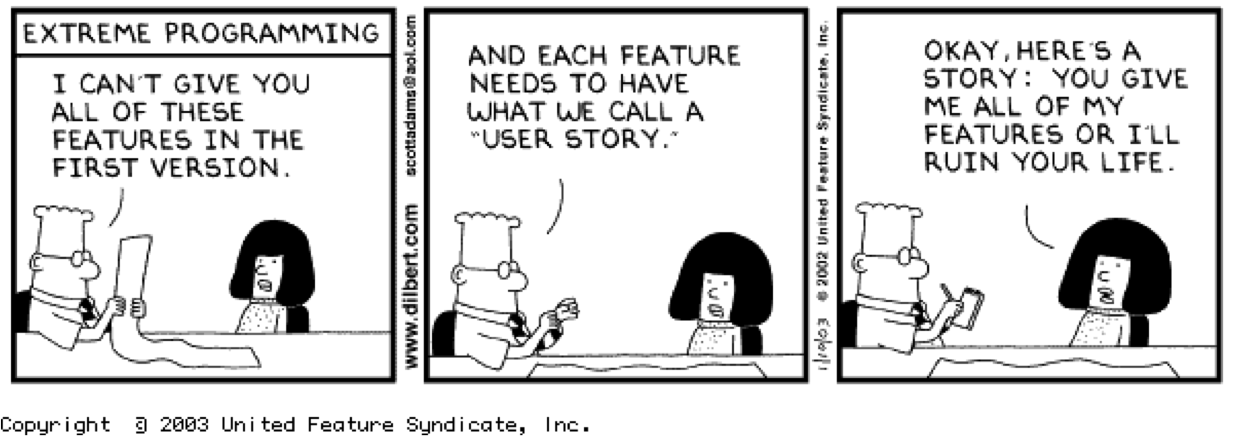
\includegraphics[width=0.8\textwidth]{images/dilbertxp2}
\end{center}
}


\frame{\frametitle{The story continues}
\begin{itemize}
\item Costing is done as a group 
\item All stories were put in the XP tracker twiki  where everyone {\em recorded the time they actually spent} on the story
\item We get better at knowing how long something actually takes. 

\item We sometimes sit at one computer but usually when there is a problem – not as a norm
\item We often sit with a projector and review code in a group ..  ..  we could do that even more often 

\end{itemize}
}


\frame{\frametitle{XP tracker twiki was used}
\begin{center}
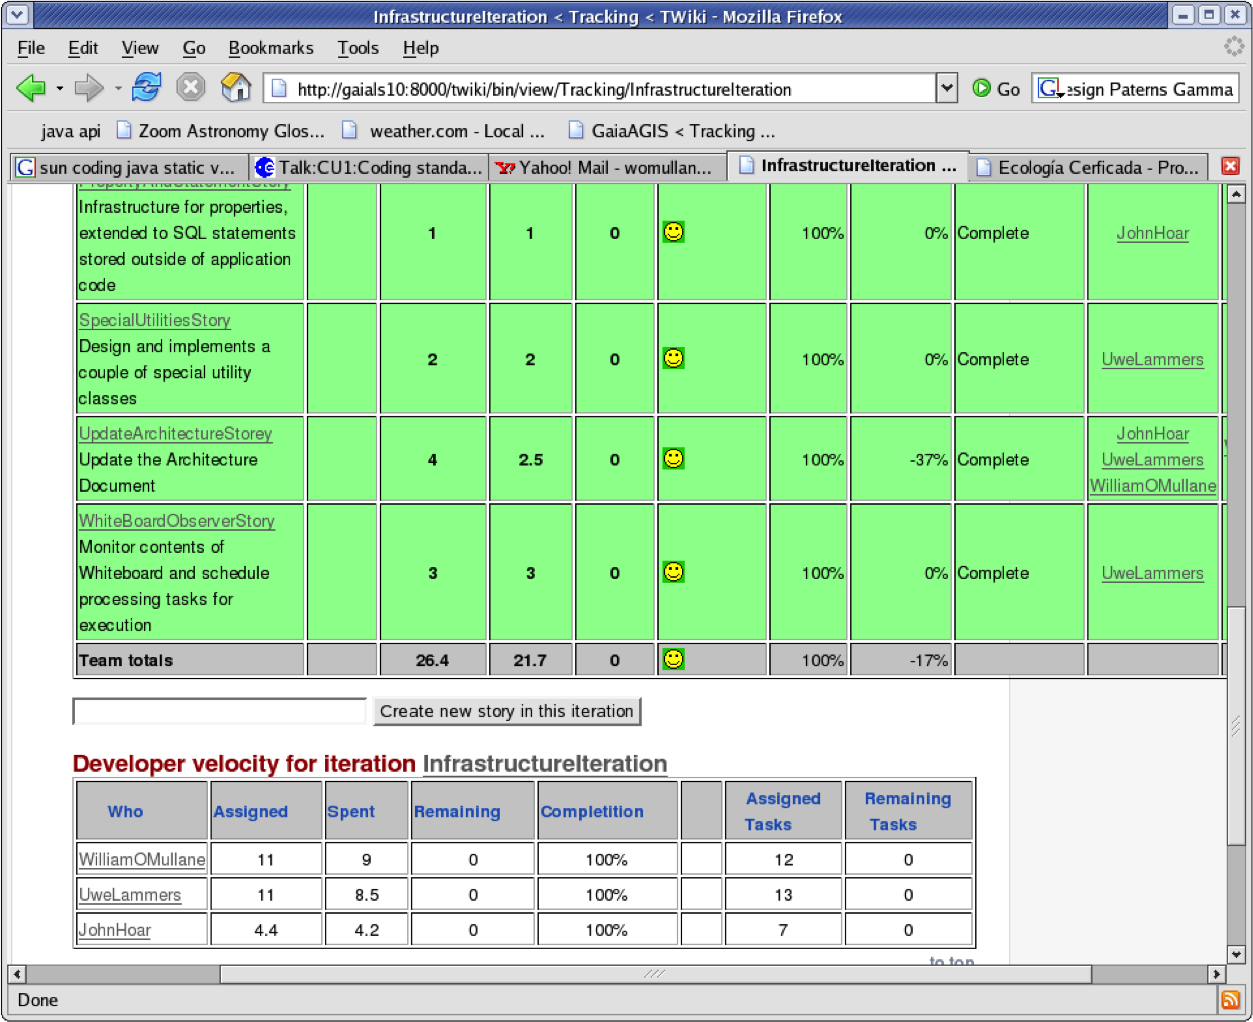
\includegraphics[width=0.8\textwidth]{images/xptracker}
\end{center}
}


\frame{\frametitle{Now we use a Google sheet }
\vspace{-10pt}
\begin{center}
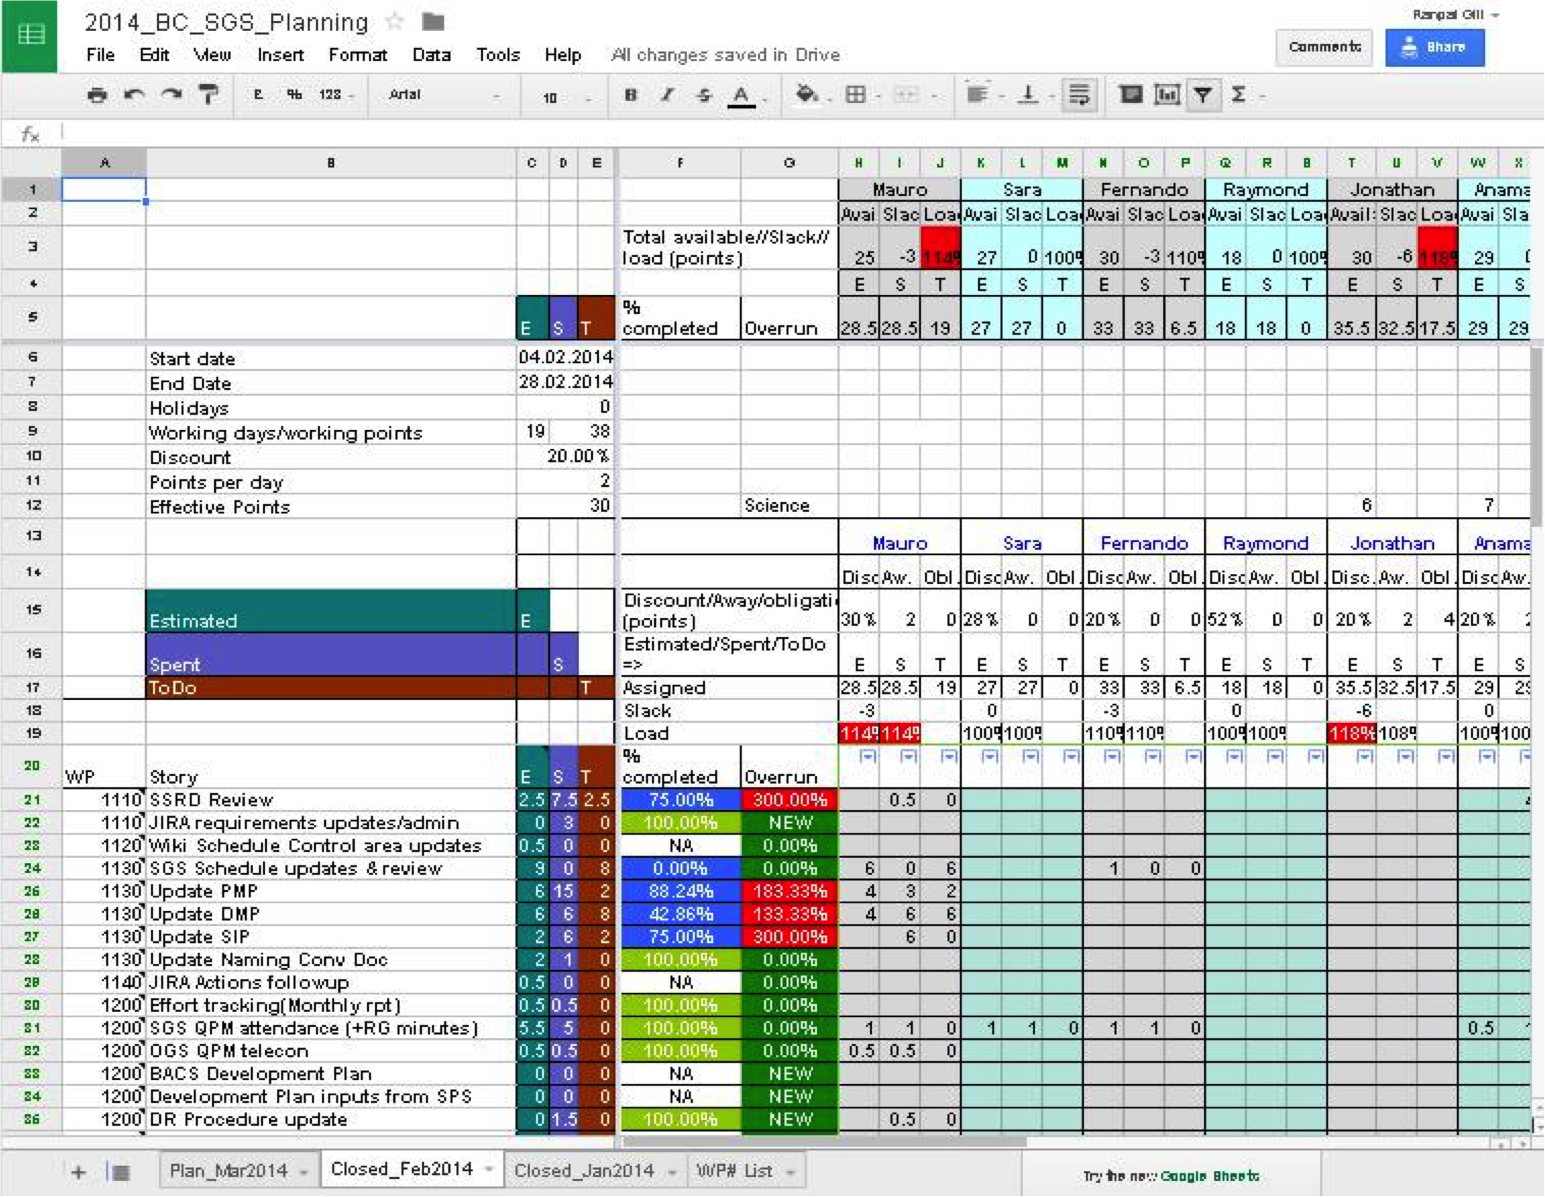
\includegraphics[width=0.85\textwidth]{images/gplan}
\end{center}
\vspace{-15pt}
{\bf \tiny from BepiColombo \citep{2014SPIE.9150E..1EG}}
}


\frame{\frametitle{Features }


We have a long term plan to launch with more firm ‘stories’ for the six month cycle we are in
\begin{itemize}
\item Work is planned in detail monthly 
\item We concentrate on what we need this month
\item We know quickly when something is much {\em tougher }than expected
\item We do not design for what we might want next year – we will do that next year
\item This keeps the code base at  a minimum 
\begin{itemize}
\item Also most code is in use !
\end{itemize}
\item This has been essential to keep system performance at peak
\begin{itemize}
\item Immediately obvious if new features slow us down.
\end{itemize}
\item Retrospective feedback 
\begin{itemize}
\item meeting had to be included as non discounted points .. 
\item meeting preparation got included 
\item science projects were included - a work package was made for that but not reported 
\end{itemize}
\end{itemize}
}

\frame{\frametitle{Why ?}

{\bf Why plan?}
\begin{itemize}
\item In a complex development enables tracking of planned schedule and better management of critical path WPs.
\item Planning:
\begin{itemize}
\item Ensures we work on what needs to be done (even the bits you don’t fancy working on!)
\item Focuses individual effort
\item Sense of accomplishment and motivation
\item Fine tuning and prioritisation of work
\end{itemize}
\end{itemize}


{\bf Why track?}
\begin{itemize}
\item Need to measure how we’re doing against the plan somehow 
\item Tracking:
\begin{itemize}
\item Monitor effort spend on WPs (defined in Cost at Completion)
\item Uncover potentially incorrect/unrealistic estimates
\item Feedback to improve planning/estimation skills
\item Progress reporting at the WP level 
\end{itemize}
\end{itemize}
}


\frame{\frametitle{Refined Process }
\begin{itemize}
\item Define period start and end dates for iteration (no points for planning meeting day ) - Set up Google sheet
\item Estimated column completed by {\color{red}controller with team members at pre-planning meeting}
\begin{itemize}
\item Points based planning per Story (WP), 1 point – 0.5 days
\item Points available are personalised by taking into account:
\begin{itemize}
\item Leave days removed
\item 20\% - 30\% discount in general since no one is 100\% productive

\item Greater discount for top management but no one can opt out 

\item Meetings, training/conference etc. fully tracked but NOT discounted

\end{itemize}
\end{itemize}
\item Spent column updated by team by end of iteration
\begin{itemize}
\item Unplanned stories can be added
\end{itemize}
\item Retrospective with whole team to look at previous \& next iteration
\item Convert points spent per story into man-month per WP
\begin{itemize}
\item Account for any sick days/unplanned leave
\end{itemize}
\item Transfer over to monthly tracking sheet generated from CaC (Cost-at-Completion) Manpower Planning (use special formula)
\begin{itemize}
\item Enables tracking of spend per WP over a period of one year
\end{itemize}
\end{itemize}
}

\frame{\frametitle{Most important TESTING}
\begin{itemize}
\item This type of approach only works with lots of test code and continuous integration
\item That means automatic tests like Junit
\begin{itemize}
\item CruiseControl builds/tests a few times a day
 \item emails everyone if the build or tests fail
\end{itemize}
\item Trying to get  >80% test coverage 
\item AGIS – just for interest 
\begin{itemize}
\item ~100K lines of code
\item ~30K lines of test code on top of that
\item ~95K lines of comments 

\end{itemize}
\end{itemize}
}


\frame{\frametitle{AGIS history}
Traditional contract with first “delivery” after 2 years still failed to produce working system after 4 years\\
 ESAC team produced first functioning AGIS within 4 months with 5 iterations

\begin{itemize}
\item Setup  - 2 weeks machines/reviewing/looking
\item Infrastructure – 2 weeks, DBMS/data access
\begin{itemize}
\item Project Scientist visit (our product owner )
\item Algo – 3 weeks, first algorithms
\begin{itemize}
\item Scientist expert visit/ pair programmed
\end{itemize}
\item Integration – 3 weeks -Underestimate 37%
\item MakeItWork – 3 weeks - refocus after missed goal
\item Test/Verification report published 
\end{itemize}
\end{itemize}


}


\frame{\frametitle{AGIS - acceptance tests}
Simulated long term basic angle variation recovered with $\mu as$ accuracy
\vspace{-5pt}
\begin{center}
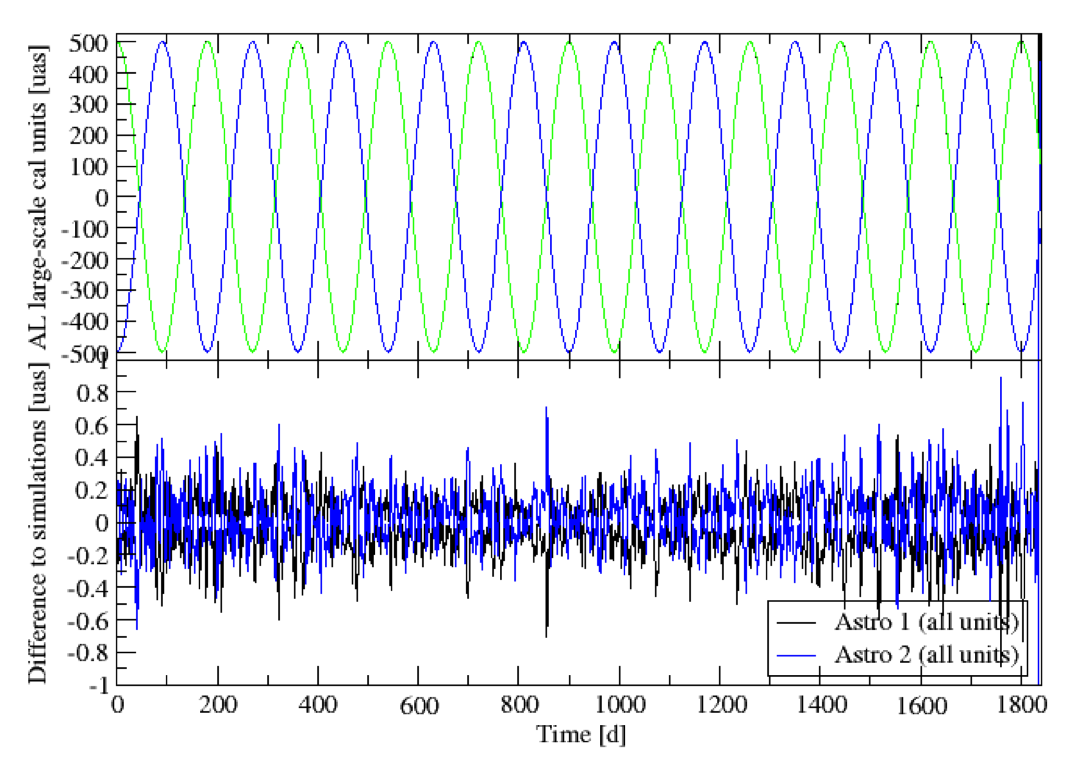
\includegraphics[width=0.8\textwidth]{images/bamrec}
\end{center}
\vspace{-5pt}
{\tiny \bf Plot from Uwe Lammers}

}



\frame{\frametitle{There there is ECSS}
{\bf European Cooperation for Space Standardization }
\begin{itemize}

\item Tells us how to do things and what documentation to produce: many books
\begin{itemize}
\item ECSS-E-10B	Requirements 
\item ECSS-M-30A	Phasing
\item ECSS-M-40B	Configuration Management
\item ECSS-Q-20B	Quality Assurance
\item …. The list is long, very long …
\item NOT unlike ITIL in this sense ..
\end{itemize}
\item Also reviews – waterfall style !
\begin{itemize}
\item Not surprising this is mainly concerned  with satellite construction.
\end{itemize}
\end{itemize}

}

\frame{\frametitle{Tailoring}
\begin{itemize}
\item ECSS actually very flexible
\begin{itemize}
\item Like that SRS etc. allow mix design and requirements great for infrastructure 
\end{itemize}
\item But that means care must be taken
\item Standard must be tailored for the project.
\item Which documents will you produce when etc …
\item Does this exist for LSST ??  -  you have some if it in LDM-493
\end{itemize}
}

\frame{\frametitle{Reviews}
\begin{itemize}
\item At least 3 or 4 before launch typically
\begin{itemize}
\item System Requirements Review
\item Critical Design Review 
\item Qualification Review 
\item Acceptance Review
\end{itemize}
\item Within DPAC there are six month development cycles – more XP style
\begin{itemize}
\item {\color{red} Docs updated in each cycle – concentration before review on docs for that review.} 
\item Latest released version of documents just pulled form the livelink and handed over - {\em no particular extra work} 
\end{itemize}
\end{itemize}
\vspace{-5pt}
\begin{center}
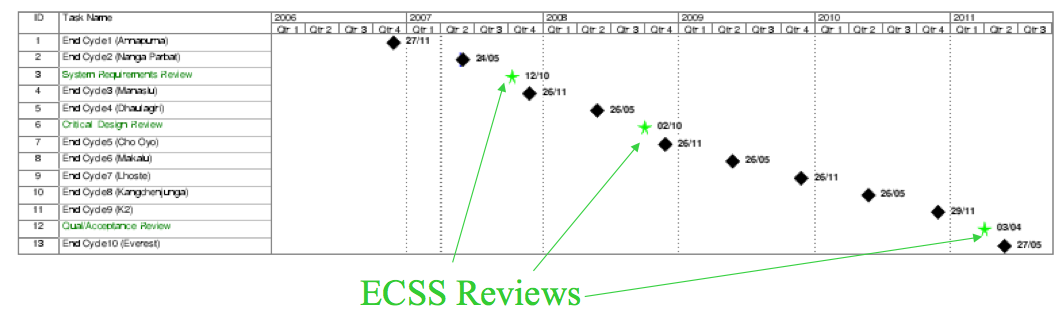
\includegraphics[width=0.8\textwidth]{images/reviews}
\end{center}
}




